\documentclass[12pt,twoside]{article}

\newcommand{\reporttitle}{477 - Computational Optimisation}
\newcommand{\reportauthor}{Jiahao Lin}
\newcommand{\reporttype}{Coursework}
\newcommand{\cid}{00837321}

% include files that load packages and define macros
%%%%%%%%%%%%%%%%%%%%%%%%%%%%%%%%%%%%%%%%%
% University Assignment Title Page 
% LaTeX Template
% Version 1.0 (27/12/12)
%
% This template has been downloaded from:
% http://www.LaTeXTemplates.com
%
% Original author:
% WikiBooks (http://en.wikibooks.org/wiki/LaTeX/Title_Creation)
%
% License:
% CC BY-NC-SA 3.0 (http://creativecommons.org/licenses/by-nc-sa/3.0/)
% 
% Instructions for using this template:
% This title page is capable of being compiled as is. This is not useful for 
% including it in another document. To do this, you have two options: 
%
% 1) Copy/paste everything between \begin{document} and \end{document} 
% starting at \begin{titlepage} and paste this into another LaTeX file where you 
% want your title page.
% OR
% 2) Remove everything outside the \begin{titlepage} and \end{titlepage} and 
% move this file to the same directory as the LaTeX file you wish to add it to. 
% Then add \input{./title_page_1.tex} to your LaTeX file where you want your
% title page.
%
%----------------------------------------------------------------------------------------
%	PACKAGES AND OTHER DOCUMENT CONFIGURATIONS
%----------------------------------------------------------------------------------------
\usepackage{ifxetex}
\usepackage{textpos}
\usepackage{natbib}
\usepackage{kpfonts}
\usepackage[a4paper,hmargin=2.8cm,vmargin=2.0cm,includeheadfoot]{geometry}
\usepackage{ifxetex}
\usepackage{stackengine}
\usepackage{tabularx,longtable,multirow,subfigure,caption}%hangcaption
\usepackage{fncylab} %formatting of labels
\usepackage{fancyhdr}
\usepackage{color}
\usepackage[tight,ugly]{units}
\usepackage{url}
\usepackage{float}
\usepackage[english]{babel}
\usepackage{amsmath}
\usepackage{graphicx}
\usepackage[colorinlistoftodos]{todonotes}
\usepackage{dsfont}
\usepackage{epstopdf} % automatically replace .eps with .pdf in graphics
\usepackage{natbib}
\usepackage{backref}
\usepackage{array}
\usepackage{latexsym}
\usepackage{etoolbox}

\usepackage{enumerate} % for numbering with [a)] format 



\ifxetex
\usepackage{fontspec}
\setmainfont[Scale=.8]{OpenDyslexic-Regular}
\else
\usepackage[pdftex,pagebackref,hypertexnames=false,colorlinks]{hyperref} % provide links in pdf
\hypersetup{pdftitle={},
  pdfsubject={}, 
  pdfauthor={\reportauthor},
  pdfkeywords={}, 
  pdfstartview=FitH,
  pdfpagemode={UseOutlines},% None, FullScreen, UseOutlines
  bookmarksnumbered=true, bookmarksopen=true, colorlinks,
    citecolor=black,%
    filecolor=black,%
    linkcolor=black,%
    urlcolor=black}
\usepackage[all]{hypcap}
\fi

\usepackage{tcolorbox}

% various theorems
\usepackage{ntheorem}
\theoremstyle{break}
\newtheorem{lemma}{Lemma}
\newtheorem{theorem}{Theorem}
\newtheorem{remark}{Remark}
\newtheorem{definition}{Definition}
\newtheorem{proof}{Proof}

% example-environment
\newenvironment{example}[1][]
{ 
\vspace{4mm}
\noindent\makebox[\linewidth]{\rule{\hsize}{1.5pt}}
\textbf{Example #1}\\
}
{ 
\noindent\newline\makebox[\linewidth]{\rule{\hsize}{1.0pt}}
}



%\renewcommand{\rmdefault}{pplx} % Palatino
% \renewcommand{\rmdefault}{put} % Utopia

\ifxetex
\else
\renewcommand*{\rmdefault}{bch} % Charter
\renewcommand*{\ttdefault}{cmtt} % Computer Modern Typewriter
%\renewcommand*{\rmdefault}{phv} % Helvetica
%\renewcommand*{\rmdefault}{iwona} % Avant Garde
\fi

\setlength{\parindent}{0em}  % indentation of paragraph

\setlength{\headheight}{14.5pt}
\pagestyle{fancy}
\fancyfoot[ER,OL]{\thepage}%Page no. in the left on
                                %odd pages and on right on even pages
\fancyfoot[OC,EC]{\sffamily }
\renewcommand{\headrulewidth}{0.1pt}
\renewcommand{\footrulewidth}{0.1pt}
\captionsetup{margin=10pt,font=small,labelfont=bf}


%--- chapter heading

\def\@makechapterhead#1{%
  \vspace*{10\p@}%
  {\parindent \z@ \raggedright %\sffamily
        %{\Large \MakeUppercase{\@chapapp} \space \thechapter}
        %\\
        %\hrulefill
        %\par\nobreak
        %\vskip 10\p@
    \interlinepenalty\@M
    \Huge \bfseries 
    \thechapter \space\space #1\par\nobreak
    \vskip 30\p@
  }}

%---chapter heading for \chapter*  
\def\@makeschapterhead#1{%
  \vspace*{10\p@}%
  {\parindent \z@ \raggedright
    \sffamily
    \interlinepenalty\@M
    \Huge \bfseries  
    #1\par\nobreak
    \vskip 30\p@
  }}
  



% %%%%%%%%%%%%% boxit
\def\Beginboxit
   {\par
    \vbox\bgroup
	   \hrule
	   \hbox\bgroup
		  \vrule \kern1.2pt %
		  \vbox\bgroup\kern1.2pt
   }

\def\Endboxit{%
			      \kern1.2pt
		       \egroup
		  \kern1.2pt\vrule
		\egroup
	   \hrule
	 \egroup
   }	

\newenvironment{boxit}{\Beginboxit}{\Endboxit}
\newenvironment{boxit*}{\Beginboxit\hbox to\hsize{}}{\Endboxit}



\allowdisplaybreaks

\makeatletter
\newcounter{elimination@steps}
\newcolumntype{R}[1]{>{\raggedleft\arraybackslash$}p{#1}<{$}}
\def\elimination@num@rights{}
\def\elimination@num@variables{}
\def\elimination@col@width{}
\newenvironment{elimination}[4][0]
{
    \setcounter{elimination@steps}{0}
    \def\elimination@num@rights{#1}
    \def\elimination@num@variables{#2}
    \def\elimination@col@width{#3}
    \renewcommand{\arraystretch}{#4}
    \start@align\@ne\st@rredtrue\m@ne
}
{
    \endalign
    \ignorespacesafterend
}
\newcommand{\eliminationstep}[2]
{
    \ifnum\value{elimination@steps}>0\leadsto\quad\fi
    \left[
        \ifnum\elimination@num@rights>0
            \begin{array}
            {@{}*{\elimination@num@variables}{R{\elimination@col@width}}
            |@{}*{\elimination@num@rights}{R{\elimination@col@width}}}
        \else
            \begin{array}
            {@{}*{\elimination@num@variables}{R{\elimination@col@width}}}
        \fi
            #1
        \end{array}
    \right]
    & 
    \begin{array}{l}
        #2
    \end{array}
    &%                                    moved second & here
    \addtocounter{elimination@steps}{1}
}
\makeatother

%% Fast macro for column vectors
\makeatletter  
\def\colvec#1{\expandafter\colvec@i#1,,,,,,,,,\@nil}
\def\colvec@i#1,#2,#3,#4,#5,#6,#7,#8,#9\@nil{% 
  \ifx$#2$ \begin{bmatrix}#1\end{bmatrix} \else
    \ifx$#3$ \begin{bmatrix}#1\\#2\end{bmatrix} \else
      \ifx$#4$ \begin{bmatrix}#1\\#2\\#3\end{bmatrix}\else
        \ifx$#5$ \begin{bmatrix}#1\\#2\\#3\\#4\end{bmatrix}\else
          \ifx$#6$ \begin{bmatrix}#1\\#2\\#3\\#4\\#5\end{bmatrix}\else
            \ifx$#7$ \begin{bmatrix}#1\\#2\\#3\\#4\\#5\\#6\end{bmatrix}\else
              \ifx$#8$ \begin{bmatrix}#1\\#2\\#3\\#4\\#5\\#6\\#7\end{bmatrix}\else
                 \PackageError{Column Vector}{The vector you tried to write is too big, use bmatrix instead}{Try using the bmatrix environment}
              \fi
            \fi
          \fi
        \fi
      \fi
    \fi
  \fi 
}  
\makeatother

\robustify{\colvec}

%%% Local Variables: 
%%% mode: latex
%%% TeX-master: "notes"
%%% End: 
 % various packages needed for maths etc.
% quick way of adding a figure
\newcommand{\fig}[3]{
 \begin{center}
 \scalebox{#3}{\includegraphics[#2]{#1}}
 \end{center}
}

%\newcommand*{\point}[1]{\vec{\mkern0mu#1}}
\newcommand{\ci}[0]{\perp\!\!\!\!\!\perp} % conditional independence
\newcommand{\point}[1]{{#1}} % points 
\renewcommand{\vec}[1]{{\boldsymbol{{#1}}}} % vector
\newcommand{\mat}[1]{{\boldsymbol{{#1}}}} % matrix
\newcommand{\R}[0]{\mathds{R}} % real numbers
\newcommand{\Z}[0]{\mathds{Z}} % integers
\newcommand{\N}[0]{\mathds{N}} % natural numbers
\newcommand{\nat}[0]{\mathds{N}} % natural numbers
\newcommand{\Q}[0]{\mathds{Q}} % rational numbers
\ifxetex
\newcommand{\C}[0]{\mathds{C}} % complex numbers
\else
\newcommand{\C}[0]{\mathds{C}} % complex numbers
\fi
\newcommand{\tr}[0]{\text{tr}} % trace
\renewcommand{\d}[0]{\mathrm{d}} % total derivative
\newcommand{\inv}{^{-1}} % inverse
\newcommand{\id}{\mathrm{id}} % identity mapping
\renewcommand{\dim}{\mathrm{dim}} % dimension
\newcommand{\rank}[0]{\mathrm{rk}} % rank
\newcommand{\determ}[1]{\mathrm{det}(#1)} % determinant
\newcommand{\scp}[2]{\langle #1 , #2 \rangle}
\newcommand{\kernel}[0]{\mathrm{ker}} % kernel/nullspace
\newcommand{\img}[0]{\mathrm{Im}} % image
\newcommand{\idx}[1]{{(#1)}}
\DeclareMathOperator*{\diag}{diag}
\newcommand{\E}{\mathds{E}} % expectation
\newcommand{\var}{\mathds{V}} % variance
\newcommand{\gauss}[2]{\mathcal{N}\big(#1,\,#2\big)} % gaussian distribution N(.,.)
\newcommand{\gaussx}[3]{\mathcal{N}\big(#1\,|\,#2,\,#3\big)} % gaussian distribution N(.|.,.)
\newcommand{\gaussBig}[2]{\mathcal{N}\left(#1,\,#2\right)} % see above, but with brackets that adjust to the height of the arguments
\newcommand{\gaussxBig}[3]{\mathcal{N}\left(#1\,|\,#2,\,#3\right)} % see above, but with brackets that adjust to the height of the arguments
\DeclareMathOperator{\cov}{Cov} % covariance (matrix) 
\ifxetex
\renewcommand{\T}[0]{^\top} % transpose
\else
\newcommand{\T}[0]{^\top}
\fi
% matrix determinant
\newcommand{\matdet}[1]{
\left|
\begin{matrix}
#1
\end{matrix}
\right|
}



%%% various color definitions
\definecolor{darkgreen}{rgb}{0,0.6,0}

\newcommand{\blue}[1]{{\color{blue}#1}}
\newcommand{\red}[1]{{\color{red}#1}}
\newcommand{\green}[1]{{\color{darkgreen}#1}}
\newcommand{\orange}[1]{{\color{orange}#1}}
\newcommand{\magenta}[1]{{\color{magenta}#1}}
\newcommand{\cyan}[1]{{\color{cyan}#1}}


% redefine emph
\renewcommand{\emph}[1]{\blue{\bf{#1}}}

% place a colored box around a character
\gdef\colchar#1#2{%
  \tikz[baseline]{%
  \node[anchor=base,inner sep=2pt,outer sep=0pt,fill = #2!20] {#1};
    }%
}%
 % short-hand notation and macros


%%%%%%%%%%%%%%%%%%%%%%%%%%%%

\begin{document}
% front page
% Last modification: Jiahao
\begin{titlepage}

\newcommand{\HRule}{\rule{\linewidth}{0.5mm}} % Defines a new command for the horizontal lines, change thickness here


%----------------------------------------------------------------------------------------


\begin{center} % Center remainder of the page

%----------------------------------------------------------------------------------------
%	HEADING SECTIONS
%----------------------------------------------------------------------------------------
\textsc{\LARGE \reporttype}\\[1.5cm] 
\textsc{\Large Imperial College London}\\[0.5cm] 
\textsc{\large Department of Computing}\\[0.5cm] 
%----------------------------------------------------------------------------------------
%	TITLE SECTION
%----------------------------------------------------------------------------------------

\HRule \\[0.4cm]
{ \huge \bfseries \reporttitle}\\ % Title of your document
\HRule \\[1.5cm]
Coursework 2
\end{center}
%----------------------------------------------------------------------------------------
%	AUTHOR SECTION
%----------------------------------------------------------------------------------------

%\begin{minipage}{0.4\hsize}
\begin{flushleft} \large
\textit{Author:}\\
\reportauthor~(CID: \cid) % Your name
\end{flushleft}
\vspace{2cm}
\makeatletter
Date: \@date 

\vfill % Fill the rest of the page with whitespace



\makeatother


\end{titlepage}




%%%%%%%%%%%%%%%%%%%%%%%%%%%% Main document
\section{Part 1}


\subsection{Q.1}


\begin{enumerate}[1)]
\item 
To prove is $\log \sum_{k=1}^{10} exp(B_{jk})$ is convex, we define:
\begin{align}
f(B_j) = \log \sum_{k=1}^{10} exp(B_{jk})\\
f(x) = \log \sum_{k=1}^{10} exp(x_k)
\end{align}
First we need to compute the Hessian of $f(x)$:
\begin{align}
\nabla f(x) = \frac{1}{1\T Z} \times z\\
\nabla^2 f(x) = \frac{1}{1\T Z} \times diag(Z) - \frac{Z\T Z}{{(1\T Z)}^2}\\
where\quad Z = \sum_{k=1}^{10} exp(x_{k})
\end{align}
For convexity we need to prove the Hessian is positive semi-definite, we need to prove:
\begin{align}
\nabla^2 f(x) \succeq 0\\
v\T\nabla^2 f(x)v >= 0\\
v\T\left(\frac{1}{1\T Z} \times diag(Z) - \frac{Z\T Z}{{(1\T Z)}^2}\right)v >= 0\\
\frac{(\sum_{k=1}^{10} Z_k V_k^2) \sum_{k=1}^{10}Z_k - \sum_{k=1}^{10}(Z_k v_k)^2}{(1\T Z)^2} >=0
\end{align}
According to Cauchy-Schwartz inequality:
\begin{align}
\sum_{k=1}^{10}(Z_k v_k)^2 \leq \sum_{k=1}^{10}Z_k \times \sum_{k=1}^{10} (Z_k V_k^2)
\end{align}
There for the Hessian is positive semi-definite holds, the Log-Sum-Exp function is convex.
\item
Denote affine mapping on $\beta_k$ as $g(\beta_k)$:
\begin{align}
g(\beta_k) = x_i\T\beta_k
\end{align}
And denote Log-Sum-Exp function as $f(x_k)$:
\begin{align}
f(x_k) = \log \sum_{k=1}^{10} exp(x_{k})
\end{align}
Now we know that $f(x_k)$ is convex, and we want to prove that $f \circ g$ is convex as well, from the definition of convexity, we need to prove:
\begin{align}
f \circ g(\alpha x + (1-\alpha)y) \leq \alpha f \circ g(x) + (1-\alpha)f \circ g(y)\\
for \quad any \quad x,\quad y \quad and\quad  \alpha \in [0,1]
\end{align}
Since we know:
\begin{align}
g(\alpha x + (1-\alpha)y) = \alpha g(x) + (1-\alpha)g(y)
\end{align}
We can prove that:
\begin{align}
f \circ g(\alpha x + (1-\alpha)y) = f ( g(\alpha x + (1-\alpha)y))\\
= f ( \alpha g(x) + (1-\alpha)g(y))\\
\leq \alpha f \circ g(x) + (1-\alpha)f \circ g(y)
\end{align}
Now we know that $\log \sum_{k=1}^{10} exp(x_i\T \beta_k)$ is convex as well.
\item
Define function $f(\beta_y)$:
\begin{align}
f(\beta_{y_i}) = -x_i\T \beta_{y_i+1}
\end{align}
We can show that:
\begin{align}
f(\alpha\beta_{x_i+1} + (1-\alpha)\beta_{y_i+1}) = -x_i\T (\alpha\beta_{x_i+1} + (1-\alpha)\beta_{y_i}+1) \\
= -\alpha x_i\T \beta_{x_i+1} - (1-\alpha)x_i\T\beta_{y_i+1}\\
= \alpha f(\beta_{x_i+1}) + (1-\alpha )f(\beta_{y_i+1})
\end{align}
Therefore $f(\beta_y)$ is convex.
\item
We can define a function for $\ell$1 Regularisation $||\beta_k||_1$:
\begin{align}
||\beta_k||_1 = f(\beta_k) = \sum_{i=1}^{N} |\beta_{ki}|
\end{align}
To prove the convexity of $f(\beta_k)$, we can show that:
\begin{align}
f(\alpha\beta_k + (1-\alpha)\beta_j) = \sum_{i=1}^{N} |\alpha\beta_k + (1-\alpha)\beta_j|\\
= \alpha\sum_{i=1}^{N} |\beta_{ki}|+ (1-\alpha)\sum_{i=1}^{N}|\beta_{ji}|\\
= \alpha f(\beta_{k})+(1-\alpha)f(\beta_{j})
\end{align}
Therefore $f(\beta_k)$ is convex.

\item
To prove the following function is convex:
\begin{align}
\sum_{i=1}^{m}\left(\log \sum_{k=1}^{10} exp(x_i\T \beta_k)-x_i\T \beta_{y_i+1}\right) + \lambda\sum_{k=1}^{10}||\beta_k||_1
\end{align}
We need to prove by decomposition, in Q2, we have shown the following term to be convex:
\begin{align}
\log \sum_{k=1}^{10} exp(x_i\T \beta_k)
\end{align}
and in Q3, we have shown the following term is convex:
\begin{align}
-x_i\T \beta_{y_i+1}
\end{align}
Therefore according to sum of convex function is also convex, we can get the sum of both is convex as well:
\begin{align}
\log \sum_{k=1}^{10} exp(x_i\T \beta_k)-x_i\T \beta_{y_i+1}
\end{align}
Following the same lemma, the summation term is also convex:
\begin{align}
\sum_{i=1}^{m}\left(\log \sum_{k=1}^{10} exp(x_i\T \beta_k)-x_i\T \beta_{y_i+1}\right)
\end{align}
In Q4, we have shown the $\ell$1 Regularisation term is convex:
\begin{align}
||\beta_k||_1
\end{align}
Then by sum of convex function is convex and affine mapping of convex function is convex, we get that the second term of optimisation problem function is convex:
\begin{align}
\lambda\sum_{k=1}^{10}||\beta_k||_1
\end{align}
Combining the convex first term and convex second term, the whole  optimisation problem is convex:
\begin{align}
\sum_{i=1}^{m}\left(\log \sum_{k=1}^{10} exp(x_i\T \beta_k)-x_i\T \beta_{y_i+1}\right) + \lambda\sum_{k=1}^{10}||\beta_k||_1
\end{align}
\end{enumerate}

\section{Part 2}
\subsection{Q.2}
\begin{enumerate}[1)]
\item
\begin{align}
h(B) = \lambda\sum_{k=1}^{10}||\beta_k||_1\\
= \lambda\sum_{k=1}^{10}\sum_{i=1}^{n}|\beta_{ik}|
\end{align}
Since absolute value is not differentiable because it has a kink at 0, the whole $h(\mathcal{B})$ function is not differentiable. So $h(\mathcal{B}) \not\in \mathcal{C}^1$.
\item
To show the new problem is convex, we need to prove that the new regularisation term is convex.
To prove the $\ell$2 regularisation term is convex, we need to show it's Hessian is positive semi-definite,
\begin{align}
||\beta_k||_2^2 = \sum_{i=1}^{10}|\beta_{k}|^2\\
= \sum_{i=1}^{10}\beta_{k}^2\\
\nabla(||\beta_k||_2^2) = Z\\
where \quad Z_k = 2\beta_k\\
\nabla^2(||\beta_k||_2^2) = diag(2)
\end{align}
Because Hessian is a diagonal matrix with all 2s on its diagonal, it's positive definite since its eigenvalues are 2 and positive eigenvalues means positive definite.\\
Now according to sum of convex function is convex and affine mapping of convex function is convex, we proved the new regularisation term is convex:
\begin{align}
\lambda\sum_{k=1}^{10}|\beta_{k}|_2^2
\end{align}
From previous question we know the first term $g(B)$ is convex, therefore the whole new optimisation problem is convex.
\begin{align}
f(B) = \sum_{i=1}^{m}\left(\log \sum_{k=1}^{10} exp(x_i\T \beta_k)-x_i\T \beta_{y_i+1}\right) + \lambda\sum_{k=1}^{10}||\beta_k||_2^2
\end{align}
We already now that the first term $g(B)$ is continuously
differentiable, and then since the new regularisation term is continuously differentiable as well because it doesn't contain the absolute function any more, we can say that the new optimisation problem $f(B) \in \mathcal{C}^1$.
\item
As shown in the code.
\item
The optimization function can be expand to first order taylor series approximation:
\begin{align}
f(B) \approx f(B_j) + \nabla f(B_j)\T(B-B_j)
\end{align}
For the algorithm to converge, we need $\delta f(B)$ tend to be zero, which can be written as:
\begin{align}
|f(B^{(j+1)}) - f(B^{(j)})| < \epsilon
\end{align}
On the other hand, if the second term tend to be zero, the condition will be met as well:
\begin{align}
\nabla f(B_j)\T(B-B_j) = 0
\end{align}
This is corresponding to the FONC (First Order Necessary Condition):
\begin{align}
\nabla f(B_j)\T d_j \leq 0
\end{align}
To satisfy the above condition, the norm of the gradient could tend to zero as well:
\begin{align}
||\nabla f(B^{(j)})||_2 < \epsilon
\end{align}
Or the change for $B$ could also tend to zero to satisfy the converge condition:
\begin{align}
||B^{(j+1)} - B^{(j)}||_2 < \epsilon
\end{align}
\item
\begin{figure}[tb]
\centering
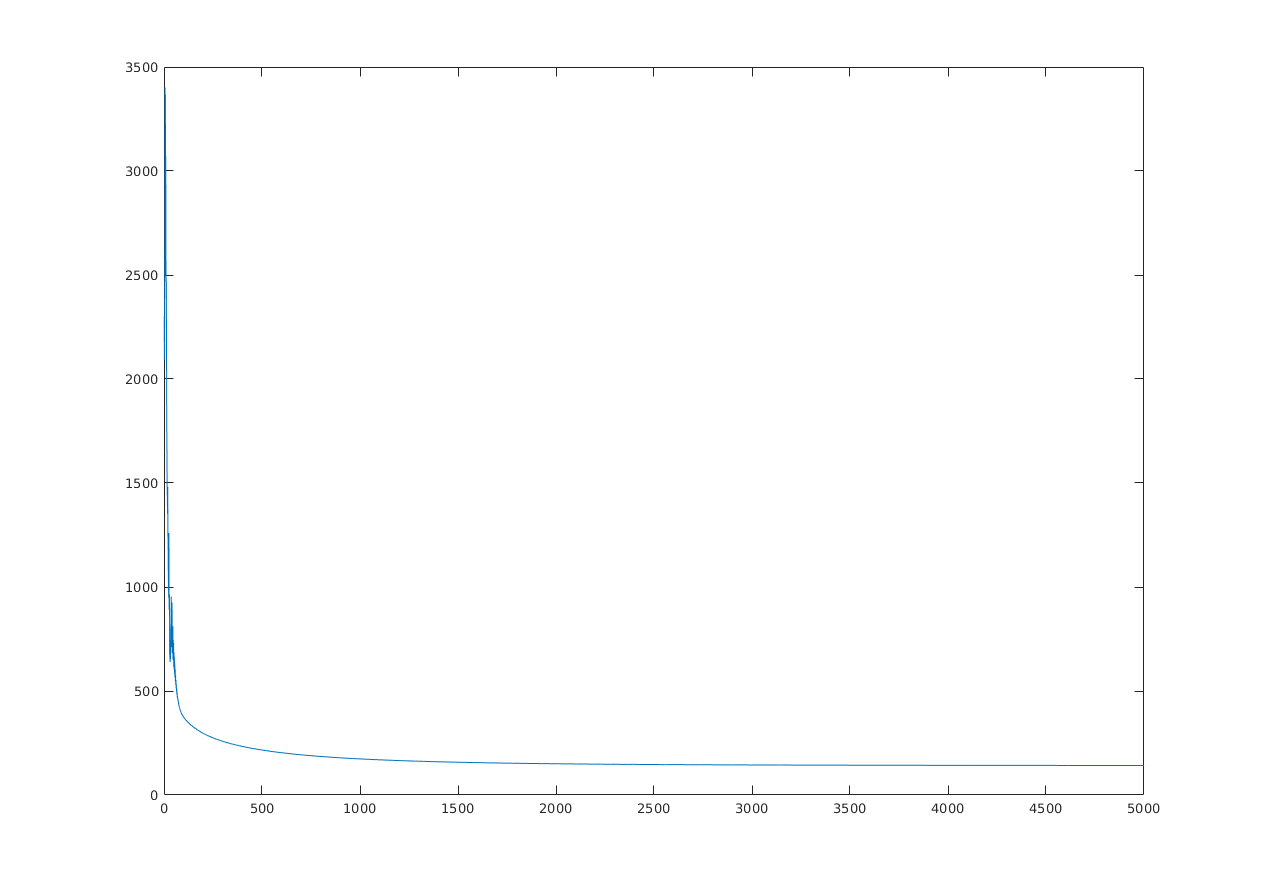
\includegraphics[width = 1.0\hsize]{./figures/p2q5}
\caption{Function values verses number of iteration using constant step size method}
\label{fig:p2q5 fig}
\end{figure}
Fig.~\ref{fig:p2q5 fig} Shows the function values verses number of iteration.\\
Result for 5000 iterations using default parameters:\\ Func Val=141.874234; FONC Residual=2.138710; Sqr Diff=0.000214
\item
The iteration of feature matrix $B$ can be written as:
\begin{align}
\beta^{j+i} = \beta^j - \alpha_j (\nabla^2 f(\beta^j))^{-1} \nabla f(\beta^j)
\end{align}
To find the optimal step size $\alpha_j$ means the minimum function value after the step, we define the problem:
 \begin{align}
\alpha_j = arg\quad min_{\alpha\geq 0} f(\beta^j - \alpha_ (\nabla^2 f(\beta^j))^{-1} \nabla f(\beta^j))
\end{align}

\item
\begin{figure}[tb]
\centering
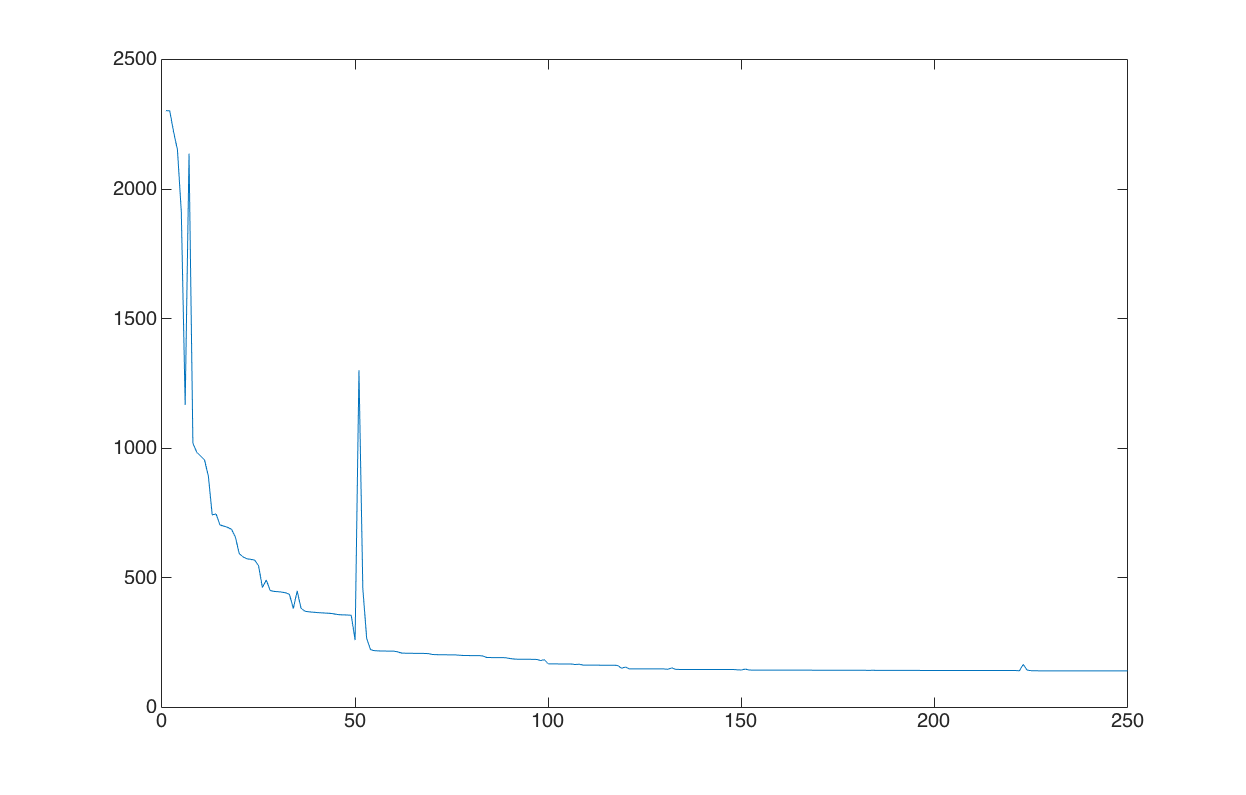
\includegraphics[width = 1.0\hsize]{./figures/secant2}
\caption{Secant method without backtrack}
\label{fig:secant2 fig}
\end{figure}
Fig.~\ref{fig:secant2 fig} Show the fast converge with secant method but not backtracking, tolerance set to 1e-8.\\
Result after 509 iterations converge: Func Val=141.231572; FONC Residual=0.002710; Sqr Diff=0.000000\\
\begin{figure}[tb]
\centering
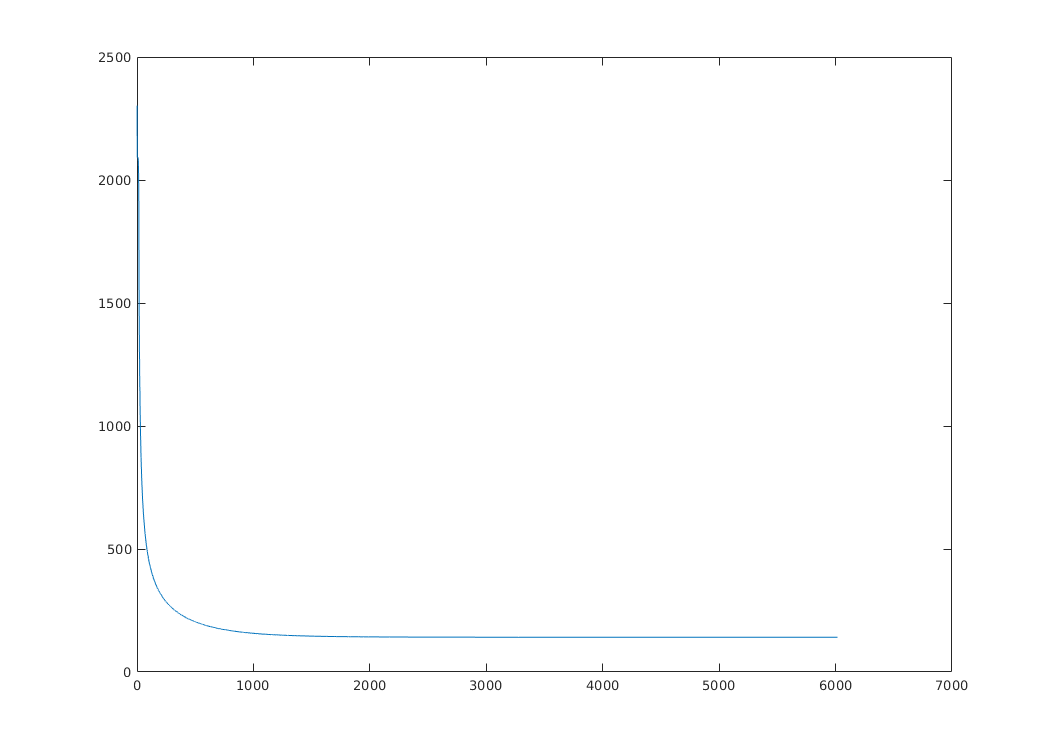
\includegraphics[width = 1.0\hsize]{./figures/final}
\caption{Secant method with backtrack}
\label{fig:secantAndBacktrack fig}
\end{figure}
Fig.~\ref{fig:secantAndBacktrack fig} Shows no converge with secant method and backtracking, tolerance set to 1e-8.\\
Result after 5000 iterations with no converge: Func Val=141.242491; FONC Residual=0.512498; Sqr Diff=0.000127\\
When leave the algorithm to run until it converges, it stopped after 6016 iterations, results are followed:\\
Func Val=141.234238; FONC Residual=0.345583; Sqr Diff=0.000075\\
\end{enumerate}

\end{document}
%%% Local Variables: 
%%% mode: latex
%%% TeX-master: t
%%% End: 
